% !TeX spellcheck = en_US
\documentclass[french]{yLectureNote}

\title{Électrocinétique}
\subtitle{Physique}
\author{Paulhenry Saux}
\date{\today}
\yLanguage{Français}

\professor{Allard}%allard@irsamc.ups-tlse.fr
\usepackage{graphicx}%----pour mettre des images
\usepackage[utf8]{inputenc}%---encodage
\usepackage{geometry}%---pour modifier les tailles et mettre a4paper
%\usepackage{awesomebox}%---pour les boites d'exercices, de pbq et de croquis ---d\'esactiv\'e pour les TP de PC
\usepackage{tikz}%---pour deiffner + d\'ependance de chemfig
\usepackage{tkz-tab}
\usepackage{chemfig}%---pour deiffner formules chimiques
\usepackage{chemformula}%---pour les formules chimiques en \'equation : \ch{...}
\usepackage{tabularx}%---pour dimensionner automatiquement les tableaux avec variable X
\usepackage{awesomebox}%---Pour les boites info, danger et autres63
\usepackage{menukeys}%---Pour deiffner les touches de Calculatrice
\usepackage{fancyhdr}%---pour les en-t\^ete personnalis\'ees
\usepackage{blindtext}%---pour les liens
\usepackage{hyperref}%---pour les liens (\`a mettre en dernier)
\usepackage{caption}%---pour la francisation de la l\'egende table vers Tableau
\usepackage{pifont}
\usepackage{array}%---pour les tableaux
\usepackage{lipsum}
\usepackage{yFlatTable}
\usepackage{multicol}
\newcommand{\Lim}[1]{\lim\limits_{\substack{#1}}\:}
\renewcommand{\vec}{\overrightarrow}
\newcommand{\dd}{\mathrm{d}}
\begin{document}
\setcounter{chapter}{5}

\chapter{Filtrage}
On prendra ce circuit en exemple dans cette fiche :

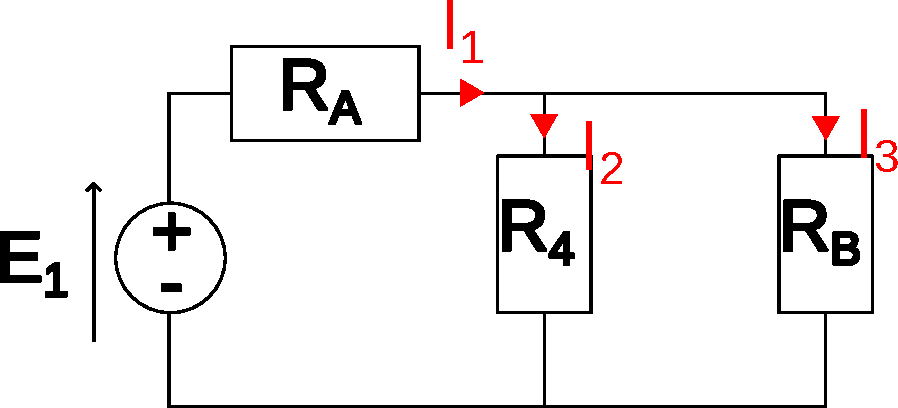
\includegraphics[scale=0.5]{path1}
\section{Détermination des fonctions utiles}
\subsection{Fonction de transfert}
\subsubsection{Impédance équivalente}

On trouve d'abord le circuit équivalent avec les impédances équivalentes, puis on applique un pont diviseur de tension.

On peut réécrire le circuit comme

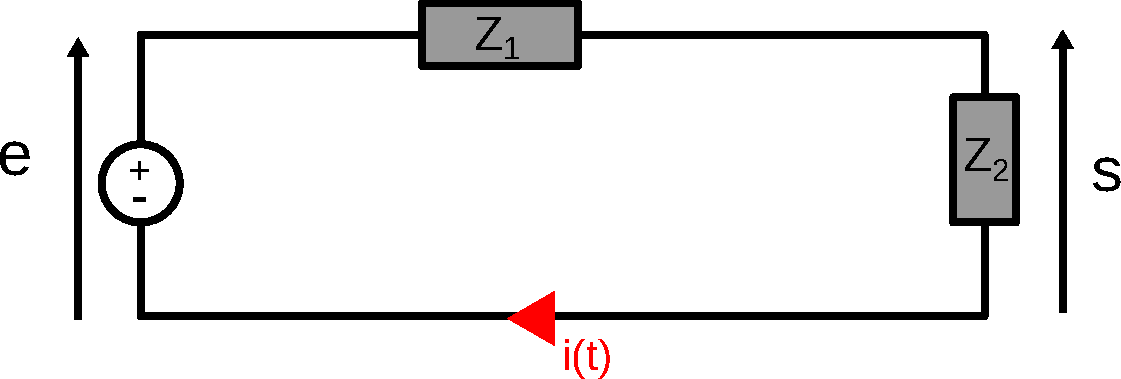
\includegraphics[scale=0.5]{equiv}


Avec, $Z_1 = jL\omega+R$ et $Z_2 = \frac{1}{\frac{1}{Z_R}+\frac{1}{Z_C}} = \frac{1}{\frac{1}{R} + jc\omega}$.

On peut maintenant exprimer s avec un pont diviseur de tension : $s = \frac{Z_2}{Z_1+Z_2}e$. Comme $H = \frac{s}{e}$, on obtient finalement que $H = \frac{1}{1+\frac{Z_1}{Z_2}}$.
\subsubsection{Forme canonique}
Pour obtenir la forme canonique avec $\omega_0$ et $Q$, on sépare les parties réelles et imaginaire, puis on identifie $\omega_0$ et $Q$.

Ici, $H = \frac{1}{2-LC\omega^2+j\omega(\frac{L}{R}+RC)} = \frac{1}{(2-(\frac{\omega}{\omega_0})^2)+j\frac{\omega}{\omega_0}(Q+\frac{1}{Q})}$ avec $\omega_0 = \frac{1}{\sqrt{LC}}$ et $Q = \frac{1}{R}\sqrt{\frac{L}{C}}$.
\subsection{Gain}
Le gain vaut le module de la fonction de transfert. Pour trouver le module de H, qui est complexe, on peut appliquer la formule (voir fiche sur les nombres complexes niveau terminale maths expertes).

\[G = \frac{1}{\sqrt{(2-(\frac{\omega}{\omega_0})^2)^2 + (\frac{\omega}{\omega_0}(Q+\frac{1}{Q}))^2 }}\]

\subsection{Gain en decibel}
On applique la formule : $G_{dB} = 20\log(G)$. Comme G est le plus souvent de la forme $\frac{1}{\sqrt{a^2+b^2}}$, on peut écrire : $G_{dB} = 20\times -\frac{1}{2} \log(a^2+b^2)$.

\subsection{Décalage de phase}
On prend l'argument de H, qui est de la forme $\frac{1}{z}$. On peut donc écrire $\varphi = -\arg(z)$. Pour trouver l'argument d'un nombre complexe, on utilise l'arctan de sa partie imaginaire sur sa partie réelle, c'est à dire : \[\arg(z) = \tan^{-1}\big(\frac{Im(z)}{Re(z)}\big)\]
\warningInfo{Négativité}{Si l'expression contenue dans arctan devient négative, il faut rajouter $\pi$ au résultat !}

Ici, $\varphi = \tan^{-1}(\frac{\frac{\omega}{\omega_0}(Q+1/Q)}{2-(\frac{\omega}{\omega_0})^2}) + \pi$ si $\omega > \sqrt{2} \omega_0$ car le dénominateur deviendrait négatif.
\section{Étude de comportements asymptotiques}
On étudie le comportement quand la pulsation tend vers 0 et vers l'infini.
\warningInfo{Comportement des bobines et condensateurs}{

À très basse fréquence, quand $\omega\to 0$, une bobine se comporte comme un fil. À l’inverse, elle se comporte comme un interrupteur ouvert quand $\omega\to\infty$.

C’est le contraire avec un condensateur, celui-ci se comporte comme un interrupteur ouvert quand $\omega\to 0$ et comme un fil quand $\omega\to\infty$.

Pour s'en rappeler, on peut imaginer le schema de la bobine s'écraser au fur et à mesure que $\omega$ est petit, jusqu' à ressembler à un fil !
}
Pour cela, on calcule la limite de H, puis celle de $G$, de $G_{dB}$ et de $\varphi$

On rappelle que $\Lim{+\infty} \arctan(x) = \frac{\pi}{2}$ et $\Lim{0} \arctan(x) = 0$.

\section{Fréquence de coupure}
% \subsection{Fréquence de coupure}

La fréquence de coupure est le plus souvent définie à -3 dB. On cherche donc la ou les pulsations telle qu'on atteint la zone de filtrage.

On cherche donc $\omega_c$ tel que $G_{dB}(\omega_c) = -3$ ou encore
\begin{flalign*}
-10 \log(a+b) &=-3= -10 \log(2)\\
\iff a+b = 2
\end{flalign*}
Comme a+b est l'expression contenant $\omega_c$, on peut le trouver en résolvant l'équation.
\criticalInfo{Filtre passe-bande}{Dans le cas du filtre passe-bande, il faut résoudre une ou plusieurs équations du second degrés. Dans ce cas, comme la pulsion est toujours positive, on ne garde que les solutions positives.}

% \subsection{Diagramme de Bode}
\section{Exemple : Filtre de Wien}
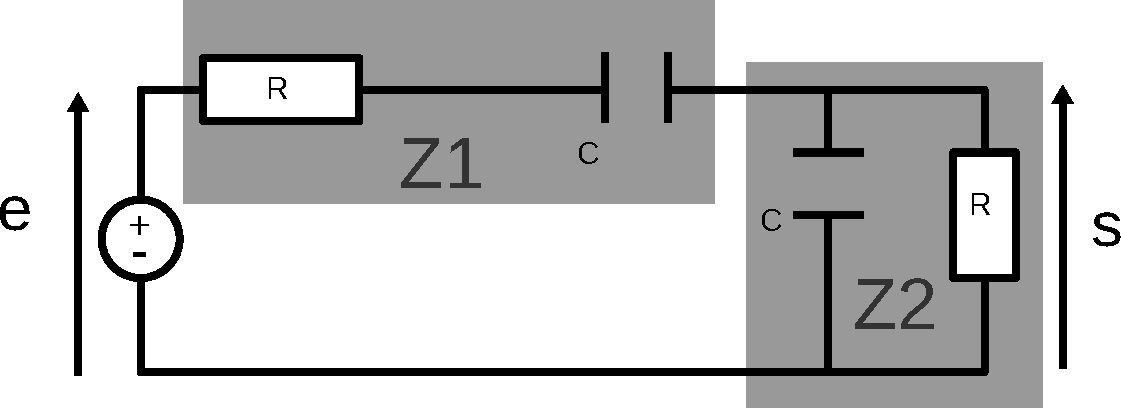
\includegraphics[scale=0.5]{wien}

Nous allons étudier la fonction de transfert de ce filtre de Wien
dans le régime sinusoïdal établi à la pulsation $\omega$.
\subsubsection{Fonction de transfert}
Montrons que la fonction de transfert peut s'écrire sous la forme \[H = \frac{A}{1+jQ(\frac{\omega}{\omega_0}-\frac{\omega_0}{\omega})}\]

On caclule le circuit équivalent avec les impédances équivalentes :
\begin{itemize}
 \item $Z_1 = R + \frac{1}{j\omega C}$
 \item $Z_2 = \frac{1}{\frac{1}{R}+ j\omega C} = \frac{R}{1 + j\omega RC}$
\end{itemize}
En appliquant un pont diviseur de tension, on trouve que H vaut \[\frac{ \frac{R}{1 + j\omega RC}}{ \frac{R}{1 + j\omega RC} + R + \frac{1}{j\omega C}}\]
\begin{flalign*}
H &= \frac{R}{1 + j\omega RC} \frac{1}{ \frac{R}{1 + j\omega RC} + R + \frac{1}{j\omega C}}\\
&= \frac{R}{ (1 + j\omega RC)(\frac{R}{1 + j\omega RC} + R + \frac{1}{j\omega C})}\\
&= \frac{R}{(\frac{R}{1 + j\omega RC} + R + \frac{1}{j\omega C}) + (j\omega CR^2 + R + \frac{jC\omega R^2}{1+j\omega RC})}\\
&= \frac{R}{2R + jC\omega R^2 + \frac{1}{j\omega C}+ \frac{R + jC\omega R^2}{1+jc\omega R}}\\
&= \frac{R}{2R + jC\omega R^2 + \frac{1}{j\omega C}+ \frac{R(1 + jC\omega R) }{1+jc\omega R}}\\
&= \frac{R}{3R + jC\omega R^2 + \frac{1}{j\omega C}}\\
&= \frac{R}{3R + jC\omega R^2 - \frac{j}{\omega C}}\\
&= \frac{R}{R(3 + j(C\omega R - \frac{1}{\omega CR}))}\\
&= \frac{1}{3 + j(C\omega R - \frac{1}{\omega CR})}\\
&= \frac{1}{3(1+ \frac{j}{3}(C\omega R - \frac{1}{\omega CR})}\\
&= \frac{\frac{1}{3}}{1+ \frac{j}{3}(C\omega R - \frac{1}{\omega CR})}\\
\end{flalign*}
On trouve bien l'expression demandée, avec $A = 1/3, Q = 1/3, \omega_0 = 1/RC$.
\subsubsection{Gain}
\begin{flalign*}
G &= |H| = |\frac{A}{1+jQ(\frac{\omega}{\omega_0}-\frac{\omega_0}{\omega})}|\\
&= \frac{|A|}{|1+jQ(\frac{\omega}{\omega_0}-\frac{\omega_0}{\omega})|}\\
&= \frac{A}{\sqrt{1+Q^2(\frac{\omega}{\omega_0}-\frac{\omega_0}{\omega})^2}}
\end{flalign*}
\begin{flalign*}
G_{dB} &= 20\log(G) = 20\log(\frac{A}{\sqrt{1+Q^2(\frac{\omega}{\omega_0}-\frac{\omega_0}{\omega})^2}})\\
&= 20\log(A) - 20\log(\sqrt{1+Q^2(\frac{\omega}{\omega_0}-\frac{\omega_0}{\omega})^2})\\
&= 20\log(A) - 10\log(1+Q^2(\frac{\omega}{\omega_0}-\frac{\omega_0}{\omega})^2)\\
\end{flalign*}
\subsubsection{Gain maximal}
\[G = \frac{A}{\sqrt{1+Q^2(\frac{\omega}{\omega_0}-\frac{\omega_0}{\omega})^2}}\]
A étant positif, le gain est maximal quand le dénomateur est le plus petit, ce qui peut se produire quand $\frac{\omega}{\omega_0}-\frac{\omega_0}{\omega} = 0$, soit quand $\omega = \omega_0$.

La valeur de $G_{dB}$ vaut alors :

\begin{flalign*}
G_{dB} &= 20\log(A) - 10\log(1+Q^2(\frac{\omega}{\omega_0}-\frac{\omega_0}{\omega})^2)\\
&= 20\log(A) - 10\log(1+Q^2(0)^2)\\
&= 20\log(A) - 10\log(1)\\
&= 20\log(A)\\
\end{flalign*}

\subsubsection{Déphasage}
\begin{flalign*}
\varphi &= \arg(H) = \arg(\frac{A}{1+jQ(\frac{\omega}{\omega_0}-\frac{\omega_0}{\omega})})\\
&= \frac{\arg(A)}{\arg(1+jQ(\frac{\omega}{\omega_0}-\frac{\omega_0}{\omega}))}\\
&= A - \arg(1+jQ(\frac{\omega}{\omega_0}-\frac{\omega_0}{\omega}))\\
&= A - \tan^{-1}(\frac{Q(\frac{\omega}{\omega_0}-\frac{\omega_0}{\omega})}{1})\\
&= A - \tan^{-1}(Q(\frac{\omega}{\omega_0}-\frac{\omega_0}{\omega})) + \pi \text{ si } \omega<\omega_0
\end{flalign*}
\subsubsection{Fréquences de coupure}
On cherche à calculer les fréquences à -3dB, c'est à dire les fréquences $\omega_{c1}, \omega_{c2}$ telles que $G_{dB}(\omega_{c1}) = G_{dB}(\omega_{c2}) = G_{dB, max} - 3$.

\begin{flalign*}
G_{dB}(\omega_{c}) &= G_{dB, max} - 3\\
&= 20\log(A) - 10\log(2)\\
&= 20\log(A) - 10\log(\sqrt{2}^2)\\
&= 20\log(A) - 20\log(\sqrt{2})\\
&= 20\log(\frac{A}{\sqrt{2}})
\end{flalign*}
De plus, \[G_{dB}(\omega_c) = 20\log(\frac{A}{\sqrt{1+Q^2(\frac{\omega_c}{\omega_0}-\frac{\omega_0}{\omega_c})^2}})\]

On en déduit que
\explanation{1}{On pose $X=\frac{\omega_c}{\omega_0}$ pour simplifier les notations}
\begin{flalign*}
&\frac{A}{\sqrt{1+Q^2(\frac{\omega_c}{\omega_0}-\frac{\omega_0}{\omega_c})^2}} = \frac{A}{\sqrt{2}}\\
&\Rightarrow 1+Q^2(\frac{\omega_c}{\omega_0}-\frac{\omega_0}{\omega_c})^2 = 2\\
&\Rightarrow Q^2(\frac{\omega_c}{\omega_0}-\frac{\omega_0}{\omega_c})^2 = 1\\
&\Rightarrow Q(\frac{\omega_c}{\omega_0}-\frac{\omega_0}{\omega_c}) = \pm 1\\
&\Rightarrow \frac{\omega_c}{\omega_0}-\frac{\omega_0}{\omega_c} = \pm \frac{1}{Q}\\
&\Rightarrow X-\frac{1}{X} = \pm \frac{1}{Q}\explain{1}{right}{0}{0.5}{×}\\
&\Rightarrow X^2-1 = \pm \frac{X}{Q}\\
&\Rightarrow X^2\pm \frac{X}{Q}-1 = 0\\
\end{flalign*}
On obtient un équation du second degré que l'on va résoudre.

$\Delta = \frac{1}{Q^2}+4>0$, donc les racines sont réelles.

On a donc
\begin{itemize}
           \item Cas $+1$ : $\displaystyle X = \frac{\frac{1}{Q}\pm \sqrt{\frac{1}{Q^2}+4}}{2}$
            \item Cas $-1$ : $\displaystyle X = \frac{-\frac{1}{Q}\pm \sqrt{\frac{1}{Q^2}+4}}{2}$
          \end{itemize}
Il y a donc 4 solutions en tout, mais on ne va garder que les racines positives. Donc

\begin{itemize}
           \item Cas $\displaystyle X_1 = \frac{\frac{1}{Q}+ \sqrt{\frac{1}{Q^2}+4}}{2}$
            \item Cas $\displaystyle X_2 = \frac{-\frac{1}{Q}+ \sqrt{\frac{1}{Q^2}+4}}{2}$
          \end{itemize}
Finalement,
\begin{itemize}
           \item $\displaystyle \omega_{c1} = \omega_0\times \frac{\frac{1}{Q}+ \sqrt{\frac{1}{Q^2}+4}}{2}$
            \item $\displaystyle \omega_{c2} =\omega_0\times \frac{-\frac{1}{Q}+ \sqrt{\frac{1}{Q^2}+4}}{2}$
          \end{itemize}
\subsubsection{Bonus : calcul de la bande passante}
\begin{flalign*}
\Delta \omega_c &= |\omega_{c1}-\omega_{c2}|\\
&= \frac{\omega_0}{Q}
\end{flalign*}
\end{document}

